% This example is meant to be compiled with lualatex or xelatex
% The theme itself also supports pdflatex
\PassOptionsToPackage{unicode}{hyperref}
\documentclass[aspectratio=1610, xcolor=dvipsnames, 9pt]{beamer}

% Load packages you need here
\usepackage{polyglossia}
\setmainlanguage{german}

\usepackage{csquotes}
\usepackage{smartdiagram}

\usepackage{amsmath}
\usepackage{amssymb}
\usepackage{mathtools}

\usepackage{hyperref}
\usepackage{bookmark}

% load the theme after all packages

\usetheme[
  showtotalframes, % show total number of frames in the footline
]{fhswf}

% Put settings here, like
\unimathsetup{
  math-style=ISO,
  bold-style=ISO,
  nabla=upright,
  partial=upright,
  mathrm=sym,
}

\title{Explainable Artificial Intelligence}
\author[F.~Neubürger]{ \textbf{Felix Neubürger}}
\institute[I \& W]{Fachhochschule Südwestfalen, Ingenieurs- \& Wirtschaftswissenschaften}
\date{2025}
\titlegraphic{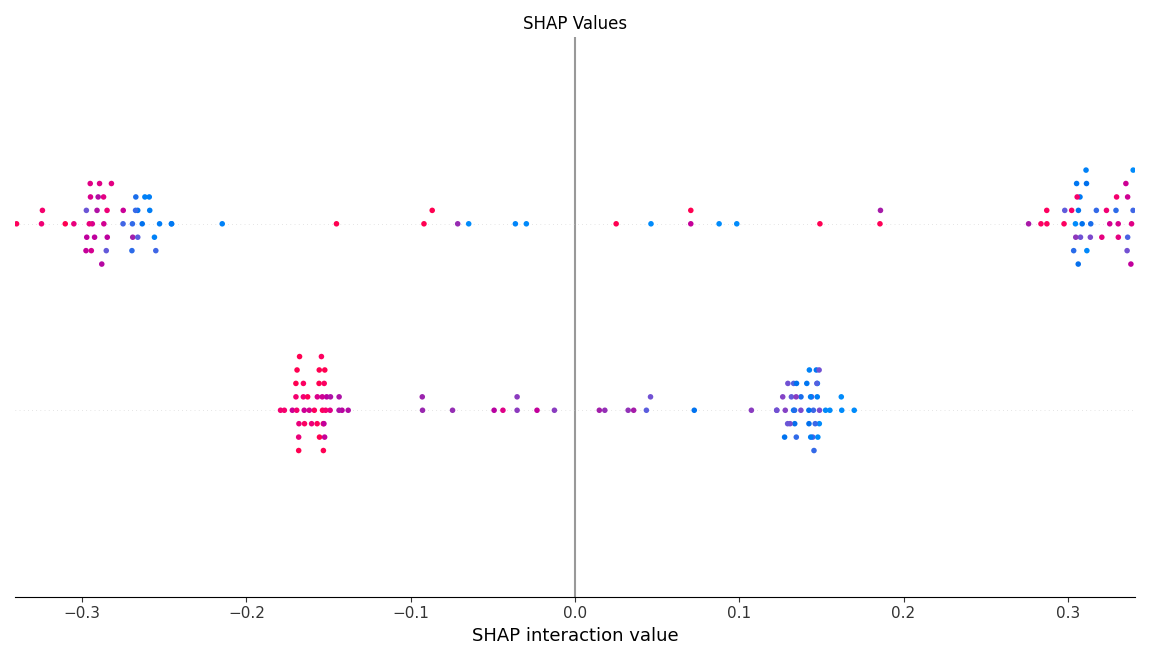
\includegraphics[width=0.6\textwidth]{images/shap_values.png}}


\begin{document}

\maketitle
\begin{frame}{Abfrage Erwartungen und Vorwissen}
  \begin{columns}
    \begin{column}{1\textwidth}
      \begin{itemize}
        \item Was verstehen Sie unter Explainable AI? \newline
        \item Haben Sie bereits Erfahrungen mit maschinellem Lernen oder KI? \newline
        \item Welche Erwartungen haben Sie an diese Vorlesung? \newline
        \item Welche Anwendungsbereiche von KI interessieren Sie besonders? \newline
        \item Gibt es spezifische Fragen, die Sie in dieser Vorlesung beantwortet haben möchten?
      \end{itemize}
    \end{column}
    \begin{column}{0\textwidth}
% \begin{figure}
% \centering
%             \includegraphics[width=0.9\textwidth]{images/intro/intro.pdf}
% \end{figure}
    \end{column}
  \end{columns}
\end{frame}

\begin{frame}{Inhalte der Vorlesung}
  \begin{columns}
    \begin{column}{1\textwidth}
      \begin{itemize}
        \item Begriffsklärungen\newline
        \item Erkenntnistheoretischer Exkurs \newline
        \item Methoden der Explainable AI  \newline
        \item Quantitative Methoden \newline 
        \item Anwendung der gelernten Methoden in einem Beispiel
      \end{itemize}
    \end{column}
    \begin{column}{0\textwidth}
% \begin{figure}
% \centering
%             \includegraphics[width=0.9\textwidth]{images/intro/intro.pdf}
% \end{figure}
    \end{column}
  \end{columns}
\end{frame}

\begin{frame}{Ziele der Vorlesung - Welche Fragen sollen beantwortet werden?}
  \begin{columns}
    \begin{column}{0.49\textwidth}
      \begin{itemize}
        \item Wofür Explainable AI? \newline
        \item Was bedeutet Explainable AI? \newline
        \item Interpretable AI?  \newline
        %\item Welche Vorteile kann Predictive Maintenance haben? \newline
        \item Trustworthy AI? \newline
        \item Wie funktioniert das mathematisch? \newline
        \item Wie schaffe ich Transparenz für Stakeholder?
        %\item Wie gehe ich an ein Predictive Maintenance Projekt heran?
      \end{itemize}
    \end{column}
    \begin{column}{0.5\textwidth}
 \begin{figure}
 \centering
             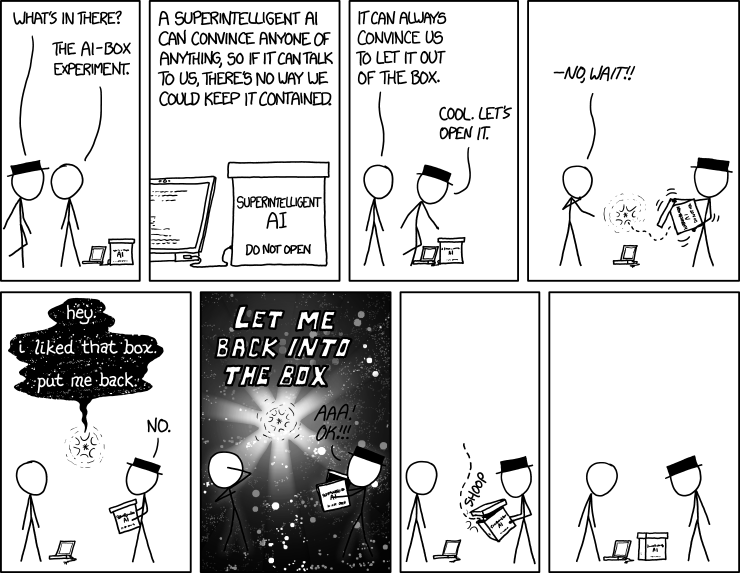
\includegraphics[width=0.9\textwidth]{images/ai_box_experiment.png}
             [\url{https://xkcd.com/1450/}]
 \end{figure}
    \end{column}
  \end{columns}
\end{frame}

\begin{frame}{Format der Vorlesung - Wie sollen diese Fragen beantwortet werden?}
  \begin{columns}
    \begin{column}{0.69\textwidth}
      \begin{itemize}
        \item Theroretischer Teil mit Folien \newline
        \item Selbststudium mt einem Lehrbuch\footnote{\url{https:// christophm.github.io/interpretable-ml-book/}} \newline
        \item Praktischer Teil in Gruppen an einem Projekt  \newline
        \item Gruppengröße 2 oder 3 Personen  \newline
        %\item Welche Vorteile kann Predictive Maintenance haben? \newline
        \item Einzelarbeit möglich wenn eigenes Thema vorhanden \newline
        \item Abgabe der Ausarbeitung einen Tag vor der Veranstaltung in der Blockwoche \newline
        \item Vorstellung der Projektergebnisse in der Blockwoche \newline
        \item Gewichtung der Bewertung Projektausarbeitung (50\%) und Vortrag (50\%)
        %
      \end{itemize}
    \end{column}
    %\begin{column}{0.3\textwidth}
 %\begin{figure}
 %\centering
 %            
\includegraphics[width=0.7\textwidth]{images/tasks.png} \newline
 %            [\url{https://xkcd.com/1425/}]
 %\end{figure}
    %\end{column}
  \end{columns}
\end{frame}

\begin{frame}{Künstliche Intelligenz (KI)}
    \begin{itemize}
        \item Teilgebiet der Informatik \newline
        \item Automatisierung intelligenten Verhaltens \newline
        \item Maschinelles Lernen als Unterbereich \newline
    \end{itemize}
\end{frame}

\begin{frame}{Maschinelles Lernen (ML)}
    \begin{itemize}
        \item Unterbereich der KI \newline
        \item Algorithmen lernen aus Daten \newline
        \item Treffen von Vorhersagen oder Entscheidungen \newline
        \item Deep Learning basiert auf künstlichen neuronalen Netzen
    \end{itemize}
\end{frame}

\begin{frame}{Explainable Artificial Intelligence (XAI)}
    \begin{itemize}
        \item Ansätze zur Verständlichkeit von KI-Entscheidungen \newline
        \item Wichtig für Vertrauen und Transparenz \newline
        \item Beispiel: Erklärungen in der medizinischen Diagnostik
    \end{itemize}
\end{frame}

\begin{frame}{Definitionen und Unterschiede}
    \begin{block}{Interpretierbarkeit}
        \begin{itemize}
            \item Fähigkeit, die internen Mechanismen eines Modells zu verstehen. 
            \item Ermöglicht direkte Einsicht in die Funktionsweise des Modells.
            \item Beispiel: Lineare Regression, Entscheidungsbäume.
        \end{itemize}
    \end{block}
    \begin{block}{Erklärbarkeit}
        \begin{itemize}
            \item Fähigkeit, die Entscheidungen oder Vorhersagen eines Modells verständlich zu machen.
            \item Oft durch zusätzliche Methoden bei komplexen Modellen erreicht.
            \item Beispiel: Neuronale Netze mit Post-hoc-Erklärungen.
        \end{itemize}
    \end{block}
\end{frame}

\begin{frame}{Erkenntnistheoretische Aspekte}
    \begin{itemize}
        \item \textbf{Wissenserwerb:} Wie tragen Interpretierbarkeit und Erklärbarkeit zum Verständnis von KI-Entscheidungen bei? \newline
        \item \textbf{Vertrauen:} Inwiefern beeinflusst die Nachvollziehbarkeit von Modellen das Vertrauen der Nutzer? \newline
        \item \textbf{Transparenz vs. Komplexität:} Balance zwischen detaillierter Einsicht und praktischer Anwendbarkeit. \newline
        \item \textbf{Ethische Verantwortung:} Bedeutung von Erklärbarkeit für ethisch vertretbare KI-Systeme. 
    \end{itemize}
\end{frame}

\begin{frame}{Bedeutung der Interpretierbarkeit im Maschinellen Lernen}
    \begin{itemize}
        \item \textbf{Definition:} \newline
        Interpretierbarkeit bezeichnet das Maß, in dem ein Mensch die Ursache einer Entscheidung eines Modells nachvollziehen kann.
        \newline
        \item \textbf{Warum ist Interpretierbarkeit wichtig?}
        \begin{itemize}
            \item \textbf{Vertrauensbildung:} \newline
            Nutzer vertrauen eher Modellen, deren Entscheidungswege sie verstehen.
            \item \textbf{Fehleranalyse:} \newline
            Verständnis für Modellentscheidungen erleichtert das Erkennen und Beheben von Fehlern.
            \item \textbf{Einhaltung gesetzlicher Vorgaben:} \newline
            In sensiblen Bereichen wie Medizin oder Finanzen sind nachvollziehbare Entscheidungen oft gesetzlich vorgeschrieben.
        \end{itemize}
    \end{itemize}
\end{frame}

\begin{frame}{Herausforderungen und Begriffsabgrenzungen}
    \begin{itemize}
        \item \textbf{Herausforderungen:}
        \begin{itemize}
            \item Fehlende einheitliche Definition von Interpretierbarkeit erschwert Kommunikation und Forschung.
            \item Kompromiss zwischen Modellkomplexität und Interpretierbarkeit oft notwendig.
        \end{itemize}
        \item \textbf{Abgrenzung zu verwandten Begriffen:}
        \begin{itemize}
            \item \textbf{Erklärbarkeit (Explainability):} \newline
            Fähigkeit, interne Mechanismen eines Modells verständlich zu machen.
            \item \textbf{Transparenz:} \newline
            Ausmaß, in dem die Funktionsweise eines Modells offenliegt.
            \item \textbf{Vertrauen:} \newline
            Maß, in dem Nutzer darauf vertrauen, dass ein Modell korrekte und faire Entscheidungen trifft.
        \end{itemize}
    \end{itemize}
\end{frame}

\begin{frame}
    \frametitle{EU-Regulierung und Erklärbare Künstliche Intelligenz}
Die Europäische Union hat den Artificial Intelligence Act verabschiedet,\footnote{Regulation (EU) 2024/1689 des Europäischen Parlaments und des Rates vom 13. Juni 2024 über harmonisierte Vorschriften für künstliche Intelligenz. Verfügbar unter: \url{https://eur-lex.europa.eu/eli/reg/2024/1689/oj}} der am 1. August 2024 in Kraft trat.\footnote{Pressemitteilung der Europäischen Kommission: "AI Act tritt in Kraft". Verfügbar unter: \url{https://ec.europa.eu/commission/presscorner/detail/de/ip_24_1234}}

    \textbf{EU AI Act: Überblick}
    \begin{itemize}
        \item \textbf{Ziel:} Einführung eines risikobasierten Klassifizierungssystems für KI-Anwendungen.  \newline
        \item \textbf{Risikokategorien:}
        \begin{itemize}
            \item \textbf{Unzulässiges Risiko:} Verbotene KI-Anwendungen.
            \item \textbf{Hohes Risiko:} Strenge Anforderungen an Transparenz, Sicherheit und Compliance.
            \item \textbf{Geringes oder minimales Risiko:} Weniger strenge oder keine spezifischen Anforderungen.
        \end{itemize}
    \end{itemize}

    \textbf{Erklärbarkeit als zentrale Anforderung} \newline
    \begin{itemize}
        \item \textbf{Transparenzpflichten:} Anbieter müssen Informationen bereitstellen, die es ermöglichen, die Funktionsweise von KI-Systemen zu verstehen.
        \item \textbf{Vertrauenswürdigkeit:} Erklärbare KI fördert das Vertrauen der Nutzer und erleichtert die Akzeptanz von KI-Technologien.
    \end{itemize}

\end{frame}

\begin{frame}
    \frametitle{Herausforderungen des EU AI Acts für Unternehmen}

    \begin{itemize}
        \item \textbf{Komplexität der Regulierung:} \\
        Der AI Act verfolgt einen risikobasierten Ansatz, bei dem KI-Systeme in verschiedene Risikoklassen eingeteilt werden. Unternehmen müssen ihre KI-Anwendungen entsprechend einstufen und die jeweiligen Anforderungen erfüllen.\footnote{\url{https://www.it-schulungen.com/wir-ueber-uns/wissensblog/welche-anforderungen-stellt-der-eu-ai-act.html}}

        \item \textbf{Standardisierung und technische Umsetzung:} \\
        Die Entwicklung harmonisierter Standards für Hochrisiko-KI-Systeme ist komplex und zeitaufwendig. Verzögerungen können zu Unsicherheiten bei der Implementierung führen und Innovationen hemmen.\footnote{\url{https://www.connect-professional.de/security/der-ai-act-chancen-nutzen-risiken-managen.332959.html}}

        \item \textbf{Vermeidung von Innovationshemmnissen:} \\
        Es besteht die Sorge, dass strenge Regulierungen Innovationen im Bereich der Künstlichen Intelligenz behindern könnten. Unternehmen müssen Wege finden, um sowohl den gesetzlichen Anforderungen zu entsprechen als auch ihre Innovationsfähigkeit zu bewahren.\footnote{\url{https://www.dps-bs.de/blog/der-ai-act-weichenstellung-fuer-kuenstliche-intelligenz-in-europa/}}

        \item \textbf{Wettbewerbsfähigkeit im internationalen Kontext:} \\
        Unternehmen in Regionen mit weniger strengen Vorschriften könnten schneller Innovationen umsetzen und dadurch Wettbewerbsvorteile erlangen. Europäische Firmen stehen vor der Herausforderung, trotz strengerer Regulierungen konkurrenzfähig zu bleiben.\footnote{\url{https://de.linkedin.com/pulse/der-eu-ai-act-chancen-und-herausforderungen-f\%C3\%BCr-andreas-quandt-ljxne}}
    \end{itemize}

\end{frame}

\begin{frame}{Methoden der Explainable AI (XAI)}
  \begin{columns}
    \begin{column}{1\textwidth}
      \textbf{Global interpretierbare Modelle:}
      \begin{itemize}
        \item Lineare Regression
        \item Entscheidungsbäume
        \item Regelbasierte Modelle
      \end{itemize}
      \vspace{0.5cm}
      \textbf{Post-hoc Erklärungen:}
      \begin{itemize}
        \item Lokale Methoden (z.B. LIME, SHAP)
        \item Visualisierungen (z.B. Feature Importance, PDPs)
        \item Gegenbeispiele (Counterfactual Explanations)
      \end{itemize}
      \vspace{0.5cm}
      \textbf{Surrogatmodelle:}
      \begin{itemize}
        \item Vereinfachte Modelle, die komplexe Modelle approximieren
      \end{itemize}
    \end{column}
    %\begin{column}{0.0\textwidth}
    %  \includegraphics[width=\textwidth]{images/xai_methods.png}
    %\end{column}
  \end{columns}
\end{frame}

\begin{frame}{Globale Methoden}
  \begin{columns}
    \begin{column}{1\textwidth}
      \textbf{Feature Importance:}
      \begin{itemize}
        \item Bewertung der Bedeutung einzelner Merkmale
      \end{itemize}
      \vspace{0.3cm}
      \textbf{Permutation Feature Importance:}
      \begin{itemize}
        \item Bewertung durch Permutation der Merkmale
      \end{itemize}
      \vspace{0.3cm}
      \textbf{Partial Dependence Plots (PDP):}
      \begin{itemize}
        \item Einfluss eines Merkmals auf die Vorhersage
      \end{itemize}
      \vspace{0.3cm}
      \textbf{Global Surrogates:}
      \begin{itemize}
        \item Erklärbares Modell, das ein komplexes Modell nachahmt
      \end{itemize}
    \end{column}
    %\begin{column}{0.4\textwidth}
    %  \includegraphics[width=\textwidth]{images/global_methods.png}
    %\end{column}
  \end{columns}
\end{frame}

\begin{frame}{Lokale Methoden}
  \begin{columns}
    \begin{column}{1\textwidth}
      \textbf{LIME:}
      \begin{itemize}
        \item Lokale lineare Approximationen des Modells
      \end{itemize}
      \vspace{0.3cm}
      \textbf{SHAP:}
      \begin{itemize}
        \item Spieltheorie-basierte Quantifizierung von Merkmalbeiträgen
      \end{itemize}
      \vspace{0.3cm}
      \textbf{Counterfactual Explanations:}
      \begin{itemize}
        \item Minimale Änderungen für eine andere Vorhersage
      \end{itemize}
    \end{column}
    %\begin{column}{0.4\textwidth}
    %  \includegraphics[width=\textwidth]{images/local_methods.png}
    %\end{column}
  \end{columns}
\end{frame}

\begin{frame}{Visualisierungen}
  \begin{columns}
    \begin{column}{1\textwidth}
      \textbf{Feature Importance:}
      \begin{itemize}
        \item Balkendiagramme zur Darstellung der Merkmalsbedeutung
      \end{itemize}
      \vspace{0.3cm}
      \textbf{Partial Dependence Plots (PDP):}
      \begin{itemize}
        \item Einfluss eines Merkmals auf die Vorhersage
      \end{itemize}
      \vspace{0.3cm}
      \textbf{Individual Conditional Expectation (ICE):}
      \begin{itemize}
        \item Individuelle Effekte von Merkmalen für einzelne Datenpunkte
      \end{itemize}
    \end{column}
    %\begin{column}{0.4\textwidth}
    %  \includegraphics[width=\textwidth]{images/visualizations.png}
    %\end{column}
  \end{columns}
\end{frame}

\begin{frame}
  \frametitle{Lineare Modelle}
  \begin{columns}
    \begin{column}{1\textwidth}
      \textbf{Lineare Regression:}
      \begin{itemize}
        \item Modell: $Y = \beta_0 + \beta_1 X_1 + \dots + \beta_p X_p + \epsilon$
        \item $\beta_0$: Achsenabschnitt
        \item $\beta_i$: Regressionskoeffizienten
        \item $\epsilon$: Fehlerterm
      \end{itemize}
      \vspace{0.5cm}
      \textbf{Generalisierte Additive Modelle (GAMs):}
      \begin{itemize}
        \item Modell: $Y = \beta_0 + f_1(X_1) + \dots + f_p(X_p) + \epsilon$
        \item $f_i$: Glatte Funktionen für nichtlineare Beziehungen
      \end{itemize}
    \end{column}
    %\begin{column}{0.4\textwidth}
    %  \includegraphics[width=\textwidth]{images/linear_models.png}
    %\end{column}
  \end{columns}
\end{frame}

\begin{frame}
  \frametitle{Entscheidungsbäume}
  \begin{columns}
    \begin{column}{0.6\textwidth}
      \begin{itemize}
        \item Rekursive Partitionierung des Merkmalsraums
        \item Jeder Knoten: Entscheidung basierend auf Merkmal und Schwellenwert
        \item Ziel: Maximierung der Homogenität in den Blättern
      \end{itemize}
    \end{column}
    \begin{column}{0.4\textwidth}
      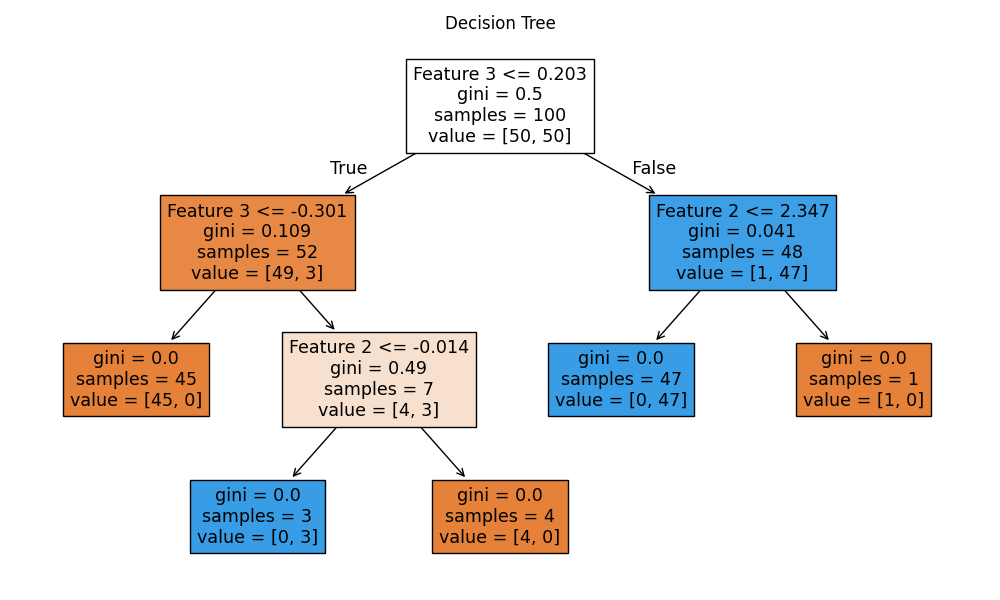
\includegraphics[width=\textwidth]{images/decision_trees.png}
    \end{column}
  \end{columns}
\end{frame}

\begin{frame}
  \frametitle{Modellagnostische Methoden}
  \begin{columns}
    \begin{column}{1\textwidth}
      \textbf{Permutation Feature Importance:}
      \begin{itemize}
        \item Permutation eines Merkmals
        \item Messung des Anstiegs des Vorhersagefehlers
        \item Signifikanter Anstieg = hohe Bedeutung
      \end{itemize}
      \vspace{0.5cm}
      \textbf{Partielle Abhängigkeitsdiagramme (PDPs):}
      \begin{itemize}
        \item Zeigen durchschnittliche Wirkung eines Merkmals
        \item Berechnung: $\hat{f}_{X_S}(x_S) = \mathbb{E}_{X_C}[\hat{f}(x_S, X_C)]$
      \end{itemize}
      \vspace{0.5cm}
      \textbf{Akkumulierte lokale Effekte (ALE):}
      \begin{itemize}
        \item Messen durchschnittliche Änderung der Vorhersage
        \item Berechnung: $ALE_j(x) = \int_{x_{min}}^x \mathbb{E} \left[ \frac{\partial \hat{f}(x)}{\partial x_j} \mid x_j = z \right] dz$
      \end{itemize}
    \end{column}
    %\begin{column}{0.4\textwidth}
    %  \includegraphics[width=\textwidth]{images/model_agnostic.png}
    %\end{column}
  \end{columns}
\end{frame}

\begin{frame}
  \frametitle{Feature Permutation Importance: Einführung}
  \begin{itemize}
    \item Ziel: Bewertung der Bedeutung eines Merkmals durch Permutation.
    \item Grundidee: Permutation eines Merkmals zerstört dessen Beziehung zur Zielvariable.
    \item Vorgehen:
    \begin{itemize}
      \item Permutiere die Werte eines Merkmals.
      \item Berechne den Anstieg des Vorhersagefehlers.
      \item Ein signifikanter Anstieg deutet auf hohe Bedeutung hin.
    \end{itemize}
  \end{itemize}
\end{frame}

\begin{frame}
  \frametitle{Feature Permutation Importance: Mathematische Berechnung}
  \begin{itemize}
    \item Gegeben:
    \begin{itemize}
      \item Modell $f$
      \item Testdatensatz $D = \{(x_i, y_i)\}_{i=1}^n$
      \item Fehlerfunktion $L(y, \hat{y})$
    \end{itemize}
    \item Berechnung:
    \begin{enumerate}
      \item Berechne den ursprünglichen Fehler:
      \[
      E_{\text{orig}} = \frac{1}{n} \sum_{i=1}^n L(y_i, f(x_i))
      \]
      \item Permutiere die Werte des Merkmals $j$: $x_j^{\text{perm}}$.
      \item Berechne den Fehler nach Permutation:
      \[
      E_{\text{perm}} = \frac{1}{n} \sum_{i=1}^n L(y_i, f(x_i^{\text{perm}}))
      \]
      \item Feature Importance:
      \[
      I_j = E_{\text{perm}} - E_{\text{orig}}
      \]
    \end{enumerate}
  \end{itemize}
\end{frame}

\begin{frame}
  \frametitle{Partial Dependence Plots (PDP): Einführung}
  \begin{itemize}
    \item Ziel: Darstellung des Einflusses eines Merkmals auf die Vorhersage.
    \item Grundidee: Durchschnittliche Vorhersage über alle anderen Merkmale hinweg.
    \item Anwendung:
    \begin{itemize}
      \item Globale Analyse von Modellen.
      \item Visualisierung nichtlinearer Beziehungen.
    \end{itemize}
  \end{itemize}
\end{frame}

\begin{frame}
  \frametitle{Partial Dependence Plots (PDP): Mathematische Berechnung}
  \begin{itemize}
    \item Gegeben:
    \begin{itemize}
      \item Modell $f$
      \item Merkmalsmenge $X = \{X_S, X_C\}$, wobei $X_S$ das zu analysierende Merkmal ist.
    \end{itemize}
    \item Berechnung:
    \[
    \hat{f}_{X_S}(x_S) = \mathbb{E}_{X_C}[f(x_S, X_C)]
    \]
    \item Diskrete Approximation:
    \[
    \hat{f}_{X_S}(x_S) \approx \frac{1}{n} \sum_{i=1}^n f(x_S, x_{C,i})
    \]
    \item Visualisierung: Plot von $\hat{f}_{X_S}(x_S)$ gegen $x_S$.
  \end{itemize}
\end{frame}

\begin{frame}
  \frametitle{Accumulated Local Effects (ALE): Einführung}
  \begin{itemize}
    \item Ziel: Messung des durchschnittlichen Einflusses eines Merkmals auf die Vorhersage.
    \item Unterschied zu PDP:
    \begin{itemize}
      \item ALE berücksichtigt die Abhängigkeiten zwischen Merkmalen.
      \item ALE ist lokaler und robuster gegenüber Korrelationen.
    \end{itemize}
  \end{itemize}
\end{frame}

\begin{frame}
  \frametitle{Accumulated Local Effects (ALE): Mathematische Berechnung}
  \begin{itemize}
    \item Gegeben:
    \begin{itemize}
      \item Modell $f$
      \item Merkmalsbereich $[x_{\text{min}}, x_{\text{max}}]$
    \end{itemize}
    \item Berechnung:
    \begin{enumerate}
      \item Berechne die lokale Wirkung:
      \[
      \Delta f(x_j, z) = \frac{\partial f(x)}{\partial x_j} \bigg|_{x_j = z}
      \]
      \item Integriere über den Bereich:
      \[
      ALE_j(x) = \int_{x_{\text{min}}}^x \mathbb{E} \left[ \Delta f(x_j, z) \mid x_j = z \right] dz
      \]
      \item Subtrahiere den Mittelwert, um zentrierte Effekte zu erhalten.
    \end{enumerate}
  \end{itemize}
\end{frame}


\begin{frame}
  \frametitle{SHAP-Werte}
  \begin{columns}
    \begin{column}{0.6\textwidth}
      \begin{itemize}
        \item Basieren auf kooperativer Spieltheorie
        \item Beitrag jedes Merkmals zur Vorhersage:
        \item $\phi_i = \sum_{S \subseteq N \setminus \{i\}} \frac{|S|! (|N| - |S| - 1)!}{|N|!} \left[ f(S \cup \{i\}) - f(S) \right]$
      \end{itemize}
    \end{column}
    \begin{column}{0.4\textwidth}
      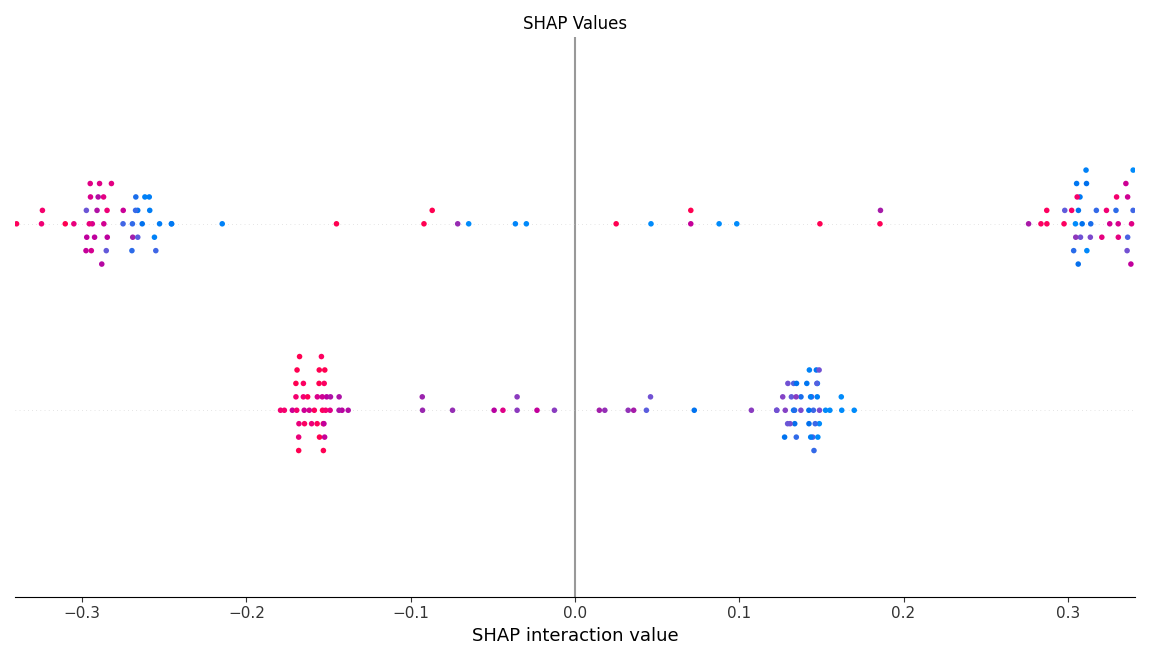
\includegraphics[width=\textwidth]{images/shap_values.png}
    \end{column}
  \end{columns}
\end{frame}

\begin{frame}
  \frametitle{SHAP-Werte: Einführung}
  \begin{itemize}
    \item \textbf{Grundlage:} 
    \begin{itemize}
      \item Basieren auf der Spieltheorie, insbesondere den Shapley-Werten.
      \item Shapley-Werte messen den durchschnittlichen marginalen Beitrag eines Spielers (Merkmals) zu einem kooperativen Spiel (Modellvorhersage).
    \end{itemize}
    \item \textbf{Eigenschaften der Shapley-Werte:}
    \begin{itemize}
      \item \textbf{Effizienz:} Die Summe aller Beiträge entspricht der Gesamtvorhersage.
      \item \textbf{Symmetrie:} Gleiche Merkmale erhalten gleiche Beiträge.
      \item \textbf{Dummy-Eigenschaft:} Merkmale ohne Einfluss haben einen Beitrag von 0.
      \item \textbf{Additivität:} Beiträge aus mehreren Modellen können kombiniert werden.
    \end{itemize}
    \item \textbf{Anwendung:}
    \begin{itemize}
      \item Erklärbarkeit von Modellvorhersagen.
      \item Identifikation der wichtigsten Merkmale.
    \end{itemize}
  \end{itemize}
\end{frame}

\begin{frame}
  \frametitle{SHAP-Werte: Berechnung (Teil 1)}
  \begin{itemize}
    \item \textbf{Formel:}
    \[
    \phi_i = \sum_{S \subseteq N \setminus \{i\}} \frac{|S|! (|N| - |S| - 1)!}{|N|!} \left[ f(S \cup \{i\}) - f(S) \right]
    \]
    \item \textbf{Erklärung der Symbole:}
    \begin{itemize}
      \item $\phi_i$: SHAP-Wert für das Merkmal $i$, der den Beitrag dieses Merkmals zur Modellvorhersage quantifiziert.
      \item $N$: Gesamte Menge aller Merkmale im Modell.
      \item $S$: Teilmenge der Merkmale aus $N$, die $i$ nicht enthält ($S \subseteq N \setminus \{i\}$).
    \end{itemize}
  \end{itemize}
\end{frame}

\begin{frame}
  \frametitle{SHAP-Werte: Berechnung (Teil 2)}
  \begin{itemize}
    \item \textbf{Erklärung der Symbole (Fortsetzung):}
    \begin{itemize}
      \item $f(S)$: Modellvorhersage, wenn nur die Merkmale in $S$ bekannt sind (andere Merkmale werden ignoriert).
      \item $f(S \cup \{i\})$: Modellvorhersage, wenn die Merkmale in $S$ sowie das Merkmal $i$ bekannt sind.
      \item $\frac{|S|! (|N| - |S| - 1)!}{|N|!}$: Gewichtungsfaktor, der die Anzahl der möglichen Reihenfolgen berücksichtigt, in denen die Merkmale in $S$ und $i$ kombiniert werden können.
    \end{itemize}
    \item \textbf{Interpretation:}
    \begin{itemize}
      \item Der SHAP-Wert $\phi_i$ misst den durchschnittlichen marginalen Beitrag des Merkmals $i$ zur Modellvorhersage über alle möglichen Teilmengen $S$.
      \item Ein positiver $\phi_i$ bedeutet, dass das Merkmal $i$ die Vorhersage erhöht, während ein negativer $\phi_i$ darauf hinweist, dass es die Vorhersage verringert.
    \end{itemize}
  \end{itemize}
\end{frame}

\begin{frame}
  \frametitle{SHAP-Werte: Vorteile}
  \begin{itemize}
    \item \textbf{Klarheit und Fairness:}
    \begin{itemize}
      \item SHAP-Werte bieten eine konsistente Methode zur Quantifizierung der Bedeutung von Merkmalen.
      \item Sie erfüllen wichtige Eigenschaften wie Effizienz und Symmetrie, was zu fairen und nachvollziehbaren Ergebnissen führt.
    \end{itemize}
    \item \textbf{Modellagnostik:}
    \begin{itemize}
      \item SHAP-Werte können für beliebige Modelle verwendet werden, unabhängig von deren Komplexität.
      \item Dies ermöglicht eine einheitliche Analyse über verschiedene Modelltypen hinweg.
    \end{itemize}
    \item \textbf{Globale und lokale Interpretierbarkeit:}
    \begin{itemize}
      \item Globale Analysen zeigen die allgemeine Bedeutung von Merkmalen.
      \item Lokale Analysen erklären spezifische Vorhersagen, was Vertrauen und Transparenz fördert.
    \end{itemize}
    \item \textbf{Spieltheoretische Grundlage:}
    \begin{itemize}
      \item Die mathematische Basis der Shapley-Werte garantiert eine robuste und theoretisch fundierte Methode.
      \item Dies stärkt die Akzeptanz in wissenschaftlichen und regulatorischen Kontexten.
    \end{itemize}
    \item \textbf{Visualisierungsmöglichkeiten:}
    \begin{itemize}
      \item SHAP-Werte können leicht visualisiert werden, z. B. durch Summary Plots oder Force Plots.
      \item Dies erleichtert die Kommunikation der Ergebnisse an Stakeholder.
    \end{itemize}
  \end{itemize}
\end{frame}

\begin{frame}
  \frametitle{Lokale Surrogatmodelle: LIME}
  \begin{columns}
    \begin{column}{0.6\textwidth}
      \begin{itemize}
        \item Einfaches Modell (z.B. lineare Regression) lokal anpassen
        \item Künstliche Datenpunkte in der Nähe generieren
        \item Gewichtung basierend auf Ähnlichkeit zur Instanz
      \end{itemize}
    \end{column}
    \begin{column}{0.4\textwidth}
      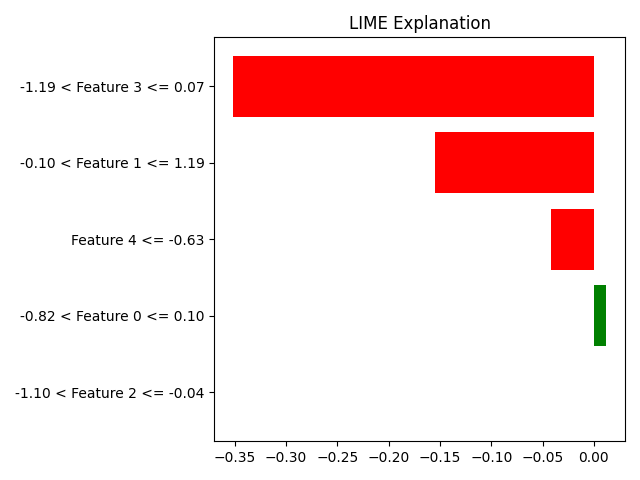
\includegraphics[width=\textwidth]{images/lime.png}
    \end{column}
  \end{columns}
\end{frame}

\begin{frame}
  \frametitle{Lokale Surrogatmodelle: Einführung in LIME}
  \begin{itemize}
    \item \textbf{Ziel:} Erklärbarkeit komplexer Modelle durch einfache, lokale Approximationen.
    \item \textbf{Grundidee:}
    \begin{itemize}
      \item Ein komplexes Modell wird in der Umgebung eines spezifischen Datenpunkts durch ein einfaches Modell (z.B. lineare Regression) approximiert.
      \item Die Approximation ist nur lokal gültig und erklärt die Vorhersage für diesen Datenpunkt.
    \end{itemize}
    \item \textbf{Vorteile:}
    \begin{itemize}
      \item Modellagnostisch: Funktioniert unabhängig vom zugrunde liegenden Modell.
      \item Flexibel: Unterstützt verschiedene Arten von Daten (tabellarisch, Text, Bilder).
    \end{itemize}
  \end{itemize}
\end{frame}

\begin{frame}
  \frametitle{LIME: Beispiel für tabellarische Daten}
  \begin{itemize}
    \item \textbf{Beispiel:} Ein Kreditbewertungsmodell sagt voraus, ob ein Kunde kreditwürdig ist.
    \item \textbf{Datenpunkt:} Ein Kunde mit folgenden Merkmalen:
    \begin{itemize}
      \item Einkommen: 50.000 €
      \item Alter: 35 Jahre
      \item Schulden: 10.000 €
    \end{itemize}
    \item \textbf{Vorhersage des Modells:} Kreditwürdig (Wahrscheinlichkeit: 85\%).
    \item \textbf{Frage:} Warum hat das Modell diese Vorhersage getroffen?
  \end{itemize}
\end{frame}

\begin{frame}
  \frametitle{LIME: Mathematisches Vorgehen (Schritt 1)}
  \textbf{Schritt 1: Generierung von Nachbardatenpunkten}
  \begin{itemize}
    \item Erzeuge künstliche Datenpunkte in der Umgebung des zu erklärenden Punktes.
    \item Beispiel: Variiere Einkommen, Alter und Schulden leicht, um ähnliche Datenpunkte zu erzeugen.
    \item Notation:
    \[
    Z = \{(x'_1, f(x'_1)), (x'_2, f(x'_2)), \dots, (x'_n, f(x'_n))\}
    \]
    wobei $x'_i$ ein Nachbardatenpunkt und $f(x'_i)$ die Vorhersage des komplexen Modells ist.
  \end{itemize}
\end{frame}

\begin{frame}
  \frametitle{LIME: Mathematisches Vorgehen (Schritt 2)}
  \textbf{Schritt 2: Gewichtung der Nachbardatenpunkte}
  \begin{itemize}
    \item Ziel: Lokale Modelle sollen die Umgebung des Originalpunkts möglichst genau beschreiben.
    \item Nahe Datenpunkte enthalten relevantere Informationen für die lokale Struktur des Modells als weiter entfernte Punkte.
    \item Berechne Gewichte basierend auf der Ähnlichkeit der Nachbardatenpunkte zum Originalpunkt.
    \item Verwende eine Distanzfunktion $d(x, x')$ und eine Kernel-Funktion $\pi(x, x')$:
    \[
    \pi(x, x') = \exp\left(-\frac{d(x, x')^2}{\sigma^2}\right)
    \]
    \item Beispiel: Für den Punkt $(50.000, 35, 10.000)$ haben Punkte mit ähnlichem Einkommen, Alter und Schulden höhere Gewichte, da sie die lokalen Eigenschaften des Modells besser repräsentieren.
  \end{itemize}
\end{frame}

\begin{frame}
  \frametitle{LIME: Mathematisches Vorgehen (Schritt 3)}
  \textbf{Schritt 3: Training des lokalen Modells}
  \begin{itemize}
    \item Trainiere ein einfaches Modell (z.B. lineare Regression) auf den gewichteten Nachbardatenpunkten.
    \item Ziel: Minimierung der gewichteten Fehlerfunktion:
    \[
    \text{Loss}(g, \pi) = \sum_{i=1}^n \pi(x, x'_i) \cdot \left(f(x'_i) - g(x'_i)\right)^2
    \]
    wobei $g$ das lokale Modell ist.
    \item Ergebnis: Ein lineares Modell, das die Vorhersage des komplexen Modells lokal approximiert.
  \end{itemize}
\end{frame}

\begin{frame}
  \frametitle{LIME: Mathematisches Vorgehen (Schritt 4)}
  \textbf{Schritt 4: Interpretation der Ergebnisse}
  \begin{itemize}
    \item Die Koeffizienten des lokalen Modells $g$ geben die Bedeutung der Merkmale an.
    \item Beispiel: Für den Punkt $(50.000, 35, 10.000)$ könnte das lokale Modell ergeben:
    \[
    g(x) = 0.3 \cdot \text{Einkommen} - 0.2 \cdot \text{Schulden} + 0.1 \cdot \text{Alter}
    \]
    \item Interpretation:
    \begin{itemize}
      \item Einkommen hat den größten positiven Einfluss auf die Vorhersage.
      \item Schulden haben einen negativen Einfluss.
      \item Alter hat einen geringeren positiven Einfluss.
    \end{itemize}
  \end{itemize}
\end{frame}

\begin{frame}
  \frametitle{Zusammenfassung: LIME}
  \begin{itemize}
    \item LIME erklärt komplexe Modelle durch einfache, lokale Approximationen.
    \item Schritte:
    \begin{enumerate}
      \item Generiere Nachbardatenpunkte.
      \item Berechne Gewichte basierend auf Ähnlichkeit.
      \item Trainiere ein einfaches Modell auf den gewichteten Daten.
      \item Interpretiere die Koeffizienten des lokalen Modells.
    \end{enumerate}
    \item Vorteile:
    \begin{itemize}
      \item Modellagnostisch und flexibel.
      \item Liefert intuitive Erklärungen für spezifische Vorhersagen.
    \end{itemize}
    \item Einschränkungen:
    \begin{itemize}
      \item Erklärungen sind nur lokal gültig.
      \item Wahl der Parameter (z.B. $\sigma$) beeinflusst die Ergebnisse.
    \end{itemize}
  \end{itemize}
\end{frame}

\begin{frame}{Zusammenfassung: Modellagnostische Erklärungsmethoden}
  \begin{table}[]
    \centering
    \begin{tabular}{|p{3cm}|p{4cm}|p{4cm}|}
      \hline
      \textbf{Methode} & \textbf{Vorteile} & \textbf{Nachteile} \\ \hline
      Permutation Feature Importance & 
      Einfache Implementierung, Modellagnostisch & 
      Kann durch Merkmalskorrelationen verzerrt werden \\ \hline
      Partial Dependence Plots (PDP) & 
      Globale Analyse, Visualisierung nichtlinearer Beziehungen & 
      Ignoriert Merkmalsabhängigkeiten \\ \hline
      Accumulated Local Effects (ALE) & 
      Robust gegenüber Merkmalskorrelationen, Lokale Analyse & 
      Schwieriger zu interpretieren als PDP \\ \hline
      SHAP-Werte & 
      Globale und lokale Interpretationen, Theoretisch fundiert & 
      Hoher Rechenaufwand bei vielen Merkmalen \\ \hline
      LIME & 
      Flexibel, Modellagnostisch, Lokale Erklärungen & 
      Erklärungen nur lokal gültig, Parameterwahl beeinflusst Ergebnisse \\ \hline
    \end{tabular}
    \caption{Zusammenfassung der modellagnostischen Erklärungsmethoden mit Vor- und Nachteilen}
  \end{table}
\end{frame}

\begin{frame}
  \frametitle{Modellabhängige Interpretationsmethoden: Einführung}
  \begin{itemize}
    \item \textbf{Definition:} 
    \begin{itemize}
      \item Modellabhängige Methoden nutzen die spezifische Struktur und Eigenschaften eines Modells, um Erklärungen zu generieren.
      \item Im Gegensatz zu modellagnostischen Methoden sind sie auf bestimmte Modelltypen zugeschnitten.
    \end{itemize}
    \item \textbf{Vorteile:}
    \begin{itemize}
      \item Höhere Präzision und Effizienz durch Nutzung von Modellwissen.
      \item Bessere Anpassung an die spezifischen Eigenschaften des Modells.
    \end{itemize}
    \item \textbf{Beispiele:}
    \begin{itemize}
      \item Gradientenbasierte Methoden (z.B. Grad-CAM, Integrated Gradients).
      \item Layer-wise Relevance Propagation (LRP).
      \item Feature Visualization für neuronale Netze.
    \end{itemize}
    \item \textbf{Anwendungsbereich:}
    \begin{itemize}
      \item Besonders relevant für komplexe Modelle wie neuronale Netze, da diese oft schwer interpretierbar sind.
    \end{itemize}
  \end{itemize}
\end{frame}

\begin{frame}
  \frametitle{Methoden zur Interpretation neuronaler Netzwerke}
  \begin{itemize}
      \item \textbf{Feature Visualization:}
      \begin{itemize}
          \item Visualisierung der Merkmale, auf die Neuronen reagieren.
          \item Ermöglicht Einblicke in die von Neuronen erkannten Muster.
      \end{itemize}
      \item \textbf{Saliency Maps:}
      \begin{itemize}
          \item Identifikation von Eingabebereichen, die den größten Einfluss auf die Ausgabe haben.
          \item Darstellung der Bedeutung einzelner Pixel oder Merkmale.
      \end{itemize}
      \item \textbf{Layer-wise Relevance Propagation (LRP):}
      \begin{itemize}
          \item Rückverfolgung der Entscheidung des Netzwerks auf die Eingabedaten.
          \item Zuweisung von Relevanzwerten zu einzelnen Eingabeelementen.
      \end{itemize}
  \end{itemize}
  \begin{figure}
      \centering
      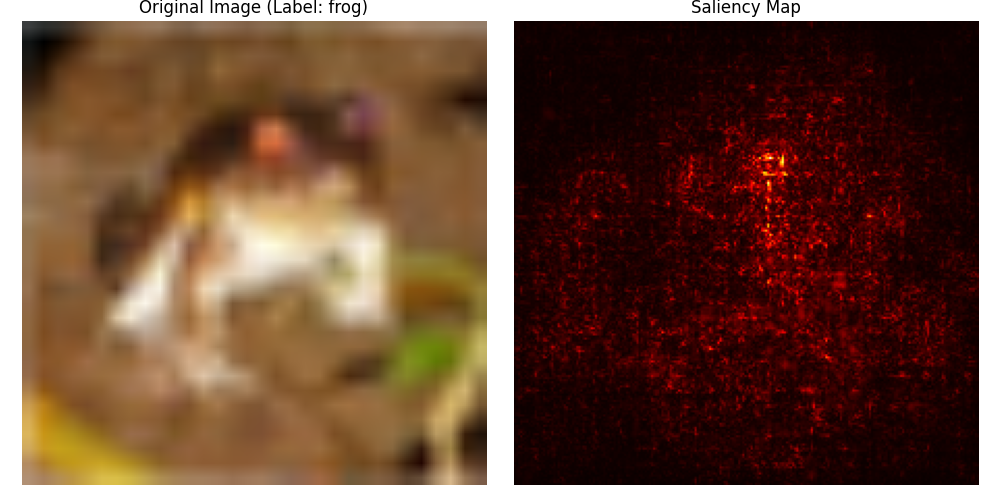
\includegraphics[width=0.5\textwidth]{images/saliency_map.png}
      \caption{Beispiel einer Saliency Map}
  \end{figure}
\end{frame}

\begin{frame}
  \frametitle{Feature Visualization: Algorithmus}
  \begin{itemize}
    \item \textbf{Ziel:} Visualisierung der Merkmale, auf die ein Neuron oder eine Schicht eines neuronalen Netzwerks reagiert.
    \item \textbf{Vorgehen:}
    \begin{enumerate}
      \item Wähle ein Neuron oder eine Schicht aus, die visualisiert werden soll.
      \item Optimiere ein Eingabebild, sodass die Aktivierung des Neurons maximiert wird.
      \item Verwende Regularisierungstechniken, um visuell interpretierbare Ergebnisse zu erhalten.
    \end{enumerate}
    \item \textbf{Warum Regularisierung?}
    \begin{itemize}
      \item Ohne Regularisierung können die optimierten Eingabebilder verrauscht oder schwer interpretierbar sein.
      \item Regularisierung hilft, visuell verständliche und interpretierbare Muster zu erzeugen.
    \end{itemize}
    \item \textbf{Anwendung:} 
    \begin{itemize}
      \item Verständnis der von einem Modell erkannten Muster.
      \item Debugging und Verbesserung von Modellen.
    \end{itemize}
  \end{itemize}
\end{frame}

\begin{frame}
  \frametitle{Feature Visualization: Mathematische Berechnung}
  \begin{itemize}
    \item \textbf{Gegeben:}
    \begin{itemize}
      \item Neuronale Aktivierung $A(x)$ für ein Eingabebild $x$.
      \item Ziel: Maximierung von $A(x)$.
    \end{itemize}
    \item \textbf{Optimierungsproblem:}
    \[
    x^* = \arg\max_x A(x) - \lambda R(x)
    \]
    \item \textbf{Erklärung der Terme:}
    \begin{itemize}
      \item $A(x)$: Aktivierung des Neurons für das Eingabebild $x$.
      \item $R(x)$: Regularisierungsterm (z.B. Total Variation, L2-Norm).
      \item $\lambda$: Gewichtung der Regularisierung.
    \end{itemize}
    \item \textbf{Lösung:}
    \begin{itemize}
      \item Gradient-basierte Optimierung (z.B. Gradient Descent).
      \item Aktualisierung des Eingabebilds:
      \[
      x \leftarrow x + \eta \frac{\partial}{\partial x} \left( A(x) - \lambda R(x) \right)
      \]
    \end{itemize}
  \end{itemize}
\end{frame}

\begin{frame}
  \frametitle{Feature Visualization: Nutzen für die Modellinterpretation}
  \begin{itemize}
    \item \textbf{Einblicke in die Funktionsweise:}
    \begin{itemize}
      \item Zeigt, welche Muster oder Merkmale ein Neuron oder eine Schicht erkennt.
      \item Hilft zu verstehen, wie das Modell Eingaben verarbeitet.
    \end{itemize}
    \item \textbf{Debugging von Modellen:}
    \begin{itemize}
      \item Identifiziert Neuronen, die auf irrelevante oder unerwartete Muster reagieren.
      \item Unterstützt bei der Verbesserung der Modellarchitektur.
    \end{itemize}
    \item \textbf{Erklärung von Entscheidungen:}
    \begin{itemize}
      \item Visualisiert, welche Merkmale zu einer bestimmten Vorhersage beitragen.
      \item Erhöht das Vertrauen in die Modellentscheidungen.
    \end{itemize}
    \item \textbf{Anwendungsbeispiele:}
    \begin{itemize}
      \item Bildklassifikation: Welche Bildbereiche sind relevant?
      \item Textverarbeitung: Welche Wörter oder Phrasen sind entscheidend?
    \end{itemize}
  \end{itemize}
\end{frame}

\begin{frame}
  \frametitle{Saliency Maps: Algorithmus}
  \begin{itemize}
    \item \textbf{Ziel:} Identifikation der Eingabebereiche, die den größten Einfluss auf die Modellvorhersage haben.
    \item \textbf{Vorgehen:}
    \begin{enumerate}
      \item Berechne den Gradienten der Modellvorhersage $f(x)$ bezüglich der Eingabe $x$.
      \item Erstelle ein Bild der absoluten Gradientenwerte.
      \item Visualisiere das Bild, um die wichtigen Bereiche hervorzuheben.
    \end{enumerate}
    \item \textbf{Anwendung:} 
    \begin{itemize}
      \item Erklärbarkeit von Bildklassifikationsmodellen.
      \item Debugging von Modellen.
    \end{itemize}
  \end{itemize}
\end{frame}

\begin{frame}
  \frametitle{Saliency Maps: Mathematische Berechnung}
  \begin{itemize}
    \item \textbf{Gegeben:}
    \begin{itemize}
      \item Modellvorhersage $f(x)$ für eine Eingabe $x$.
    \end{itemize}
    \item \textbf{Berechnung:}
    \[
    S(x) = \left| \frac{\partial f(x)}{\partial x} \right|
    \]
    \item \textbf{Erklärung der Terme:}
    \begin{itemize}
      \item $\frac{\partial f(x)}{\partial x}$: Gradient der Vorhersage $f(x)$ bezüglich der Eingabe $x$.
      \item $S(x)$: Saliency Map, die die Bedeutung jedes Pixels oder Merkmals zeigt.
    \end{itemize}
    \item \textbf{Beispiel:}
    \begin{itemize}
      \item Für ein Bild $x$ mit Pixelwerten berechne den Gradienten $\frac{\partial f(x)}{\partial x}$.
      \item Erstelle eine Heatmap basierend auf den absoluten Werten der Gradienten.
    \end{itemize}
  \end{itemize}
\end{frame}


\begin{frame}
  \frametitle{Layer-wise Relevance Propagation (LRP): Algorithmus}
  \begin{itemize}
    \item \textbf{Ziel:} Rückverfolgung der Modellvorhersage auf die Eingabedaten, um die Relevanz jedes Eingabeelements zu bestimmen.
    \item \textbf{Vorgehen:}
    \begin{enumerate}
      \item Beginne mit der Modellvorhersage $f(x)$.
      \item Verteile die Relevanz schichtweise rückwärts durch das Netzwerk.
      \item Nutze Relevanzverteilungsregeln, um die Relevanz auf die Eingabedaten zu projizieren.
    \end{enumerate}
    \item \textbf{Anwendung:} 
    \begin{itemize}
      \item Erklärbarkeit von neuronalen Netzwerken.
      \item Identifikation wichtiger Eingabemerkmale.
    \end{itemize}
  \end{itemize}
\end{frame}

\begin{frame}
  \frametitle{Layer-wise Relevance Propagation (LRP): Mathematische Berechnung}
  \begin{itemize}
    \item \textbf{Gegeben:}
    \begin{itemize}
      \item Neuronale Aktivierungen $z_{ij}$ zwischen Neuronen $i$ und $j$.
      \item Relevanz $R_j$ eines Neurons $j$ in der nächsten Schicht.
    \end{itemize}
    \item \textbf{Startwert der Relevanz:}
    \begin{itemize}
      \item Die Relevanz $R_j$ in der Ausgangsschicht entspricht der Modellvorhersage $f(x)$:
      \[
      R_j = f(x)
      \]
    \end{itemize}
    \item \textbf{Relevanzverteilung:}
    \[
    R_i = \sum_j \frac{z_{ij}}{\sum_k z_{kj}} R_j
    \]
    \item \textbf{Erklärung der Terme:}
    \begin{itemize}
      \item $z_{ij}$: Beitrag des Neurons $i$ zum Neuron $j$.
      \item $\sum_k z_{kj}$: Gesamte Eingabe zum Neuron $j$.
      \item $R_i$: Relevanz des Neurons $i$.
    \end{itemize}
    \item \textbf{Beispiel:}
    \begin{itemize}
      \item Für ein neuronales Netzwerk mit Eingabe $x$ und Vorhersage $f(x)$ wird die Relevanz von $f(x)$ schichtweise auf die Eingabe $x$ zurückgeführt.
    \end{itemize}
  \end{itemize}
\end{frame}

\begin{frame}
  \frametitle{Layer-wise Relevance Propagation (LRP): Interpretation einzelner Schichten}
  \begin{itemize}
    \item \textbf{Ziel:} Analyse der Relevanzverteilung in jeder Schicht des neuronalen Netzwerks.
    \item \textbf{Vorgehen:}
    \begin{itemize}
      \item Rückverfolgung der Relevanz von der Ausgangsschicht bis zur Eingabeschicht.
      \item Untersuchung der Relevanzverteilung in jeder Zwischenschicht.
    \end{itemize}
    \item \textbf{Nutzen:}
    \begin{itemize}
      \item Identifikation der Schichten, die am meisten zur Vorhersage beitragen.
      \item Verständnis der Informationsverarbeitung im Netzwerk.
    \end{itemize}
  \end{itemize}
\end{frame}

\begin{frame}
  \frametitle{LRP: Interpretation der Zwischenschichten}
  \begin{itemize}
    \item \textbf{Relevanz in Zwischenschichten:}
    \begin{itemize}
      \item Jede Schicht erhält Relevanzwerte basierend auf ihrer Aktivierung und ihrem Beitrag zur nächsten Schicht.
      \item Relevanzverteilung zeigt, welche Neuronen in einer Schicht besonders wichtig sind.
    \end{itemize}
    \item \textbf{Beispiel:}
    \begin{itemize}
      \item In einer Convolutional Layer können Relevanzwerte zeigen, welche Filter die wichtigsten Merkmale extrahieren.
      \item In einer Fully Connected Layer können sie die Bedeutung einzelner Neuronen quantifizieren.
    \end{itemize}
    \item \textbf{Visualisierung:}
    \begin{itemize}
      \item Heatmaps oder Diagramme können verwendet werden, um die Relevanz in jeder Schicht darzustellen.
    \end{itemize}
  \end{itemize}
\end{frame}

\begin{frame}
  \frametitle{LRP: Vorteile der Schichtweisen Analyse}
  \begin{itemize}
    \item \textbf{Einblicke in die Modellstruktur:}
    \begin{itemize}
      \item Verstehen, wie Informationen durch das Netzwerk fließen.
      \item Identifikation von Schichten, die für spezifische Aufgaben entscheidend sind.
    \end{itemize}
    \item \textbf{Debugging:}
    \begin{itemize}
      \item Erkennen von Schichten, die irrelevante oder fehlerhafte Informationen verarbeiten.
      \item Verbesserung der Netzwerkarchitektur basierend auf den Relevanzanalysen.
    \end{itemize}
    \item \textbf{Erklärbarkeit:}
    \begin{itemize}
      \item Transparenz für Stakeholder durch detaillierte Erklärungen der Modellentscheidungen.
      \item Erhöhtes Vertrauen in die Vorhersagen des Modells.
    \end{itemize}
  \end{itemize}
\end{frame}

\begin{frame}
  \frametitle{Grad-CAM: Einführung}
  \begin{itemize}
    \item \textbf{Ziel:} Visualisierung der relevanten Bildbereiche, die zu einer Modellvorhersage beitragen.
    \item \textbf{Grundidee:}
    \begin{itemize}
      \item Grad-CAM nutzt die Gradienten der Zielklasse, um die Bedeutung der Feature-Maps einer Convolutional Layer zu bestimmen.
      \item Die resultierende Heatmap zeigt, welche Bildbereiche für die Vorhersage am wichtigsten sind.
    \end{itemize}
    \item \textbf{Anwendungsbereiche:}
    \begin{itemize}
      \item Bildklassifikation: Identifikation relevanter Bildbereiche.
      \item Medizinische Bildanalyse: Lokalisierung von Anomalien.
      \item Debugging von CNNs: Überprüfung, ob das Modell auf sinnvolle Merkmale achtet.
    \end{itemize}
  \end{itemize}
\end{frame}

\begin{frame}
  \frametitle{Grad-CAM: Schritt 1 - Gradientenberechnung}
  \begin{itemize}
    \item \textbf{Ziel:} Berechnung der Gradienten der Zielklasse $y^c$ bezüglich der Feature-Maps $A^k$ einer Convolutional Layer.
    \item \textbf{Formel:}
    \[
    \frac{\partial y^c}{\partial A_{ij}^k}
    \]
    \item \textbf{Erklärung:}
    \begin{itemize}
      \item $y^c$: Modellvorhersage für die Zielklasse $c$.
      \item $A^k$: Feature-Map $k$ der ausgewählten Convolutional Layer.
      \item $\frac{\partial y^c}{\partial A_{ij}^k}$: Gradient der Zielklasse $y^c$ bezüglich der Aktivierung an Position $(i, j)$ in der Feature-Map $A^k$.
    \end{itemize}
    \item \textbf{Nutzen:} Die Gradienten zeigen, wie stark die Aktivierungen in $A^k$ die Zielklasse beeinflussen.
  \end{itemize}
\end{frame}

\begin{frame}
  \frametitle{Grad-CAM: Schritt 2 - Gewichtung der Feature-Maps}
  \begin{itemize}
    \item \textbf{Ziel:} Aggregation der Gradienten über die räumlichen Dimensionen, um die Bedeutung jeder Feature-Map zu bestimmen.
    \item \textbf{Formel:}
    \[
    \alpha_k^c = \frac{1}{Z} \sum_{i} \sum_{j} \frac{\partial y^c}{\partial A_{ij}^k}
    \]
    \item \textbf{Erklärung:}
    \begin{itemize}
      \item $\alpha_k^c$: Gewicht für die Feature-Map $A^k$ in Bezug auf die Zielklasse $c$.
      \item $Z$: Anzahl der räumlichen Positionen in der Feature-Map $A^k$.
      \item $\sum_{i} \sum_{j}$: Summe über alle räumlichen Positionen $(i, j)$.
    \end{itemize}
    \item \textbf{Nutzen:} Die Gewichte $\alpha_k^c$ geben an, wie wichtig jede Feature-Map für die Zielklasse ist.
  \end{itemize}
\end{frame}

\begin{frame}
  \frametitle{Grad-CAM: Schritt 3 - Erzeugung der Heatmap}
  \begin{itemize}
    \item \textbf{Ziel:} Erstellung der Grad-CAM Heatmap durch gewichtete Kombination der Feature-Maps.
    \item \textbf{Formel:}
    \[
    L_{\text{Grad-CAM}}^c = \text{ReLU}\left(\sum_k \alpha_k^c A^k\right)
    \]
    \item \textbf{Erklärung:}
    \begin{itemize}
      \item $\alpha_k^c$: Gewicht der Feature-Map $A^k$ für die Zielklasse $c$.
      \item $\sum_k$: Summe über alle Feature-Maps.
      \item $\text{ReLU}$: Aktivierungsfunktion, um negative Werte zu entfernen.
    \end{itemize}
    \item \textbf{Nutzen:} Die resultierende Heatmap $L_{\text{Grad-CAM}}^c$ zeigt die relevanten Bildbereiche für die Zielklasse.
  \end{itemize}
\end{frame}

\begin{frame}
  \frametitle{Grad-CAM: Zusammenfassung und Vorteile}
  \begin{itemize}
    \item \textbf{Zusammenfassung:}
    \begin{enumerate}
      \item Berechne die Gradienten der Zielklasse $y^c$ bezüglich der Feature-Maps $A^k$.
      \item Aggregiere die Gradienten, um die Gewichte $\alpha_k^c$ zu bestimmen.
      \item Erstelle die Grad-CAM Heatmap durch gewichtete Kombination der Feature-Maps.
    \end{enumerate}
    \item \textbf{Vorteile:}
    \begin{itemize}
      \item Intuitive Visualisierung der relevanten Bildbereiche.
      \item Modellagnostisch für Convolutional Neural Networks (CNNs).
      \item Unterstützt Debugging und Verbesserung von Modellen.
    \end{itemize}
    \item \textbf{Anwendungsbeispiele:}
    \begin{itemize}
      \item Bildklassifikation: Identifikation der wichtigsten Bildbereiche.
      \item Medizinische Bildanalyse: Lokalisierung von Anomalien.
    \end{itemize}
  \end{itemize}
\end{frame}

\begin{frame}
  \frametitle{Grad-CAM: Herausforderungen}
  \begin{itemize}
    \item \textbf{Herausforderungen:}
    \begin{itemize}
      \item Bei Modellen wie RCNNs, die nicht durchgängig differenzierbar sind, können Gradientenberechnungen problematisch sein.
      \item Nicht-differenzierbare Operationen (z. B. ROI-Pooling) führen zu ungenauen oder fehlenden Gradienten.
      \item Mögliche Lösung: Approximationstechniken oder modifizierte Varianten von Grad-CAM.
    \end{itemize}
  \end{itemize}
\end{frame}

\begin{frame}
  \frametitle{Integrated Gradients: Einführung}
  \begin{itemize}
    \item \textbf{Ziel:} Quantifizierung des Beitrags jedes Eingabemerkmals zur Modellvorhersage.
    \item \textbf{Grundidee:}
    \begin{itemize}
      \item Integriere die Gradienten der Modellvorhersage entlang eines geraden Pfads von einer Baseline-Eingabe $x'$ zur aktuellen Eingabe $x$.
    \end{itemize}
    \item \textbf{Formel:}
    \[
    \text{IG}_i(x) = (x_i - x'_i) \int_{\alpha=0}^1 \frac{\partial f(x' + \alpha (x - x'))}{\partial x_i} d\alpha
    \]
    \item \textbf{Eigenschaften:}
    \begin{itemize}
      \item \textbf{Pfadinvarianz:} Die Summe der Beiträge entspricht der Differenz der Modellvorhersagen zwischen $x$ und $x'$.
      \item \textbf{Baseline:} Die Wahl der Baseline (z.B. Nullvektor) beeinflusst die Ergebnisse.
    \end{itemize}
  \end{itemize}
\end{frame}


\begin{frame}
  \frametitle{Integrated Gradients: Detaillierte Berechnung}
  \begin{itemize}
    \item \textbf{Gegeben:}
    \begin{itemize}
      \item Eingabe $x$ und Baseline $x'$ (z. B. Nullvektor oder Durchschnittswerte).
      \item Modellvorhersage $f(x)$.
    \end{itemize}
    \item \textbf{Schritte:}
    \begin{enumerate}
      \item \textbf{Pfaddefinition:} Definiere einen geraden Pfad von $x'$ nach $x$:
      \[
      x(\alpha) = x' + \alpha (x - x'), \quad \alpha \in [0, 1]
      \]
      \item \textbf{Gradientenberechnung:} Berechne den Gradienten der Modellvorhersage entlang des Pfads:
      \[
      \frac{\partial f(x(\alpha))}{\partial x_i}
      \]
      \item \textbf{Integration:} Integriere die Gradienten entlang des Pfads:
      \[
      \text{IG}_i(x) = (x_i - x'_i) \int_{\alpha=0}^1 \frac{\partial f(x(\alpha))}{\partial x_i} d\alpha
      \]
    \end{enumerate}
    \item \textbf{Numerische Approximation:}
    \begin{itemize}
      \item Diskretisiere den Pfad in $m$ Schritte: $\alpha_1, \alpha_2, \dots, \alpha_m$.
      \item Approximiere das Integral durch eine Summe:
      \[
      \text{IG}_i(x) \approx (x_i - x'_i) \cdot \frac{1}{m} \sum_{k=1}^m \frac{\partial f(x(\alpha_k))}{\partial x_i}
      \]
    \end{itemize}
  \end{itemize}
\end{frame}

\begin{frame}
  \frametitle{Integrated Gradients: Anwendungszwecke}
  \begin{itemize}
    \item \textbf{Anwendungsbereiche:}
    \begin{itemize}
      \item \textbf{Bildklassifikation:} Identifikation der Pixel, die am meisten zur Vorhersage beitragen.
      \item \textbf{Textverarbeitung:} Bewertung der Bedeutung einzelner Tokens oder Wörter.
      \item \textbf{Tabellarische Daten:} Analyse der Merkmalsbeiträge für spezifische Vorhersagen.
    \end{itemize}
    \item \textbf{Vorteile:}
    \begin{itemize}
      \item Modellagnostisch: Funktioniert für beliebige differenzierbare Modelle.
      \item Robust gegenüber kleinen Änderungen in den Eingabedaten.
    \end{itemize}
    \item \textbf{Beispiele:}
    \begin{itemize}
      \item Medizinische Diagnostik: Identifikation relevanter Merkmale in Patientendaten.
      \item Finanzwesen: Erklärung von Kreditentscheidungen.
    \end{itemize}
  \end{itemize}
\end{frame}

\begin{frame}{Zusammenfassung: Methoden der Explainable AI}
  \begin{table}[]
    \centering
    \begin{tabular}{|p{2.5cm}|p{3.5cm}|p{3.5cm}|p{3.5cm}|}
      \hline
      \textbf{Methode} & \textbf{Vorteile} & \textbf{Nachteile} & \textbf{Anwendungsfälle} \\ \hline
      Grad-CAM & 
      Intuitive Visualisierung relevanter Bildbereiche & 
      Funktioniert nur für CNNs, Probleme bei nicht-differenzierbaren Modellen & 
      Bildklassifikation, Medizinische Bildanalyse \\ \hline
      Integrated Gradients & 
      Robust, Modellagnostisch & 
      Wahl der Baseline beeinflusst Ergebnisse & 
      Bilder, Text, Tabellarische Daten \\ \hline
      Layer-wise Relevance Propagation (LRP) & 
      Schichtweise Analyse, Rückverfolgbarkeit & 
      Abhängig von Modellarchitektur & 
      Neuronale Netzwerke \\ \hline
    \end{tabular}
    \caption{Zusammenfassung der XAI-Methoden mit Vor- und Nachteilen sowie Anwendungsfällen}
  \end{table}
\end{frame}

\begin{frame}
  \frametitle{Werkzeuge und Bibliotheken für XAI}
  \begin{itemize}
      \item \textbf{Captum:}
      \begin{itemize}
          \item PyTorch-Bibliothek für Interpretierbarkeitsmethoden.
          \item Unterstützt Techniken wie integrierte Gradienten und DeepLIFT.
      \end{itemize}
      \item \textbf{ELI5:}
      \begin{itemize}
          \item Bibliothek zur Erklärung von ML-Modellen und Vorhersagen.
          \item Unterstützt verschiedene Modelle wie Sklearn, XGBoost und Keras.
      \end{itemize}
      \item \textbf{SHAP-Bibliothek:}
      \begin{itemize}
          \item Implementierung der SHAP-Werte für verschiedene Modelltypen.
          \item Ermöglicht detaillierte Analysen der Merkmalsbeiträge.
      \end{itemize}
  \end{itemize}
  \begin{figure}
      \centering
        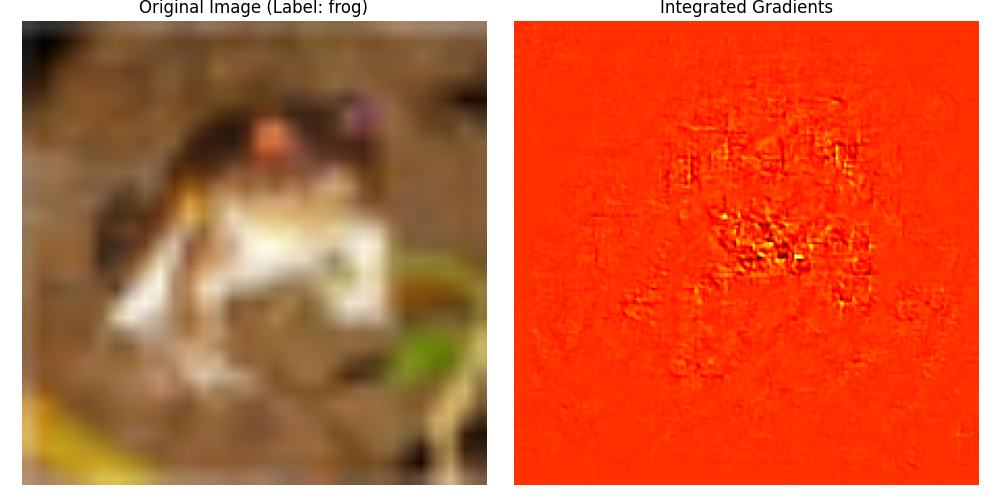
\includegraphics[width=0.5\textwidth]{images/integrated_gradients.png}
        \caption{Integrated Gradients zur Modellinterpretation}
  \end{figure}
\end{frame}

\begin{frame}{Erklärung für Sentiment-Analyse mit LLM}
  \begin{columns}
    \begin{column}{0.6\textwidth}
      \begin{itemize}
        \item \textbf{Ziel:} Generierung und Speicherung einer Erklärung für eine Sentiment-Analyse-Aufgabe.
        \item \textbf{Vorgehen:}
        \begin{itemize}
          \item Verwendung eines vortrainierten Sprachmodells (LLM) aus der Hugging Face Transformers-Bibliothek.
          \item Durchführung der Sentiment-Analyse auf einem Beispieltext.
          \item Visualisierung der Erklärung (z.B. Token-Wichtigkeit) als Balkendiagramm.
        \end{itemize}
        \item \textbf{Ergebnis:} 
        \begin{itemize}
          \item Die Bedeutung einzelner Tokens wird grafisch dargestellt, um die Entscheidungsfindung des Modells zu verdeutlichen.
        \end{itemize}
      \end{itemize}
    \end{column}
    \begin{column}{0.4\textwidth}
      \begin{figure}
        \centering
        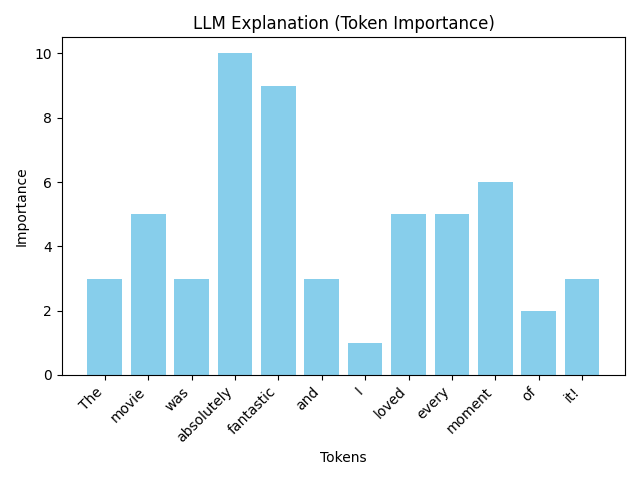
\includegraphics[width=\textwidth]{images/sentiment_explanation.png}
        \caption{Visualisierung der Token-Wichtigkeit für Sentiment-Analyse}
      \end{figure}
    \end{column}
  \end{columns}
\end{frame}

\begin{frame}{Interpretation von LLMs (Large Language Models)}
  \begin{itemize}
    \item \textbf{Herausforderungen:}
    \begin{itemize}
      \item Hohe Komplexität und Anzahl der Parameter erschweren die Nachvollziehbarkeit.
      \item Entscheidungen basieren auf nichtlinearen Beziehungen zwischen Tokens.
    \end{itemize}
    \item \textbf{Ansätze zur Interpretation:}
    \begin{itemize}
      \item \textbf{Attention Visualisierung:}
      \begin{itemize}
        \item Darstellung der Aufmerksamkeit (Attention Scores) zwischen Tokens.
        \item Tool: BertViz.
      \end{itemize}
      \item \textbf{Feature Attribution:}
      \begin{itemize}
        \item Identifikation der wichtigsten Tokens für eine Vorhersage.
        \item Tools: Captum, SHAP.
      \end{itemize}
      \item \textbf{Neuronale Aktivierungen:}
      \begin{itemize}
        \item Analyse der Aktivierungsmuster einzelner Neuronen.
        \item Tool: Neuroscope.
      \end{itemize}
    \end{itemize}
  \end{itemize}
\end{frame}

\begin{frame}
  \frametitle{Interpretation von LLMs: Attention Visualisierung}
  \begin{itemize}
    \item \textbf{Ziel:} Darstellung der Aufmerksamkeit (Attention Scores) zwischen Tokens.
    \item \textbf{Grundidee:}
    \begin{itemize}
      \item Transformer-Modelle wie BERT und GPT nutzen Attention-Mechanismen, um die Beziehungen zwischen Tokens zu modellieren.
      \item Die Attention-Matrix zeigt, wie stark ein Token auf andere Tokens achtet.
    \end{itemize}
    \item \textbf{Beispiel:}
    \begin{itemize}
      \item Satz: "The cat sat on the mat."
      \item Visualisierung: Zeigt, dass "cat" stark mit "sat" und "mat" verbunden ist.
    \end{itemize}
    \item \textbf{Werkzeuge:}
    \begin{itemize}
      \item BertViz: Interaktive Visualisierung der Attention-Matrizen.
    \end{itemize}
  \end{itemize}
\end{frame}

\begin{frame}
  \frametitle{Attention Visualisierung: Algorithmus}
  \begin{itemize}
    \item \textbf{Schritt 1: Berechnung der Attention-Matrix}
    \begin{itemize}
      \item Gegeben: Eingabe-Tokens $x_1, x_2, \dots, x_n$.
      \item Berechnung der Attention-Werte:
      \[
      \text{Attention}(Q, K, V) = \text{softmax}\left(\frac{QK^T}{\sqrt{d_k}}\right)V
      \]
      \item $Q, K, V$: Query-, Key- und Value-Matrizen.
      \item $d_k$: Dimension der Key-Vektoren.
    \end{itemize}
    \item \textbf{Schritt 2: Extraktion der Attention Scores}
    \begin{itemize}
      \item Die Attention-Matrix enthält die Scores für jedes Token-Paar.
      \item Beispiel: Attention von "cat" auf "sat" beträgt 0.8.
    \end{itemize}
    \item \textbf{Schritt 3: Visualisierung}
    \begin{itemize}
      \item Erstelle eine Heatmap, um die Scores darzustellen.
      \item Höhere Werte werden durch intensivere Farben hervorgehoben.
    \end{itemize}
  \end{itemize}
\end{frame}

\begin{frame}
  \frametitle{Interpretation von LLMs: Feature Attribution}
  \begin{itemize}
    \item \textbf{Ziel:} Identifikation der wichtigsten Tokens für eine Vorhersage.
    \item \textbf{Ansatz:}
    \begin{itemize}
      \item Quantifiziere den Beitrag jedes Tokens zur Modellvorhersage.
      \item Nutze Methoden wie Integrated Gradients oder SHAP.
    \end{itemize}
    \item \textbf{Beispiel:}
    \begin{itemize}
      \item Satz: "The movie was absolutely fantastic."
      \item Ergebnis: "fantastic" hat den höchsten Beitrag zur positiven Sentiment-Vorhersage.
    \end{itemize}
    \item \textbf{Werkzeuge:}
    \begin{itemize}
      \item Captum: Unterstützt Integrated Gradients.
      \item SHAP: Berechnet Shapley-Werte für Tokens.
    \end{itemize}
  \end{itemize}
\end{frame}

\begin{frame}
  \frametitle{Feature Attribution: Algorithmus (Integrated Gradients)}
  \begin{itemize}
    \item \textbf{Schritt 1: Definition der Baseline}
    \begin{itemize}
      \item Wähle eine Baseline-Eingabe $x'$ (z. B. leere Tokens).
    \end{itemize}
    \item \textbf{Schritt 2: Berechnung der Gradienten}
    \begin{itemize}
      \item Definiere einen Pfad von der Baseline $x'$ zur Eingabe $x$:
      \[
      x(\alpha) = x' + \alpha (x - x'), \quad \alpha \in [0, 1]
      \]
      \item Berechne die Gradienten entlang des Pfads:
      \[
      \frac{\partial f(x(\alpha))}{\partial x_i}
      \]
    \end{itemize}
    \item \textbf{Schritt 3: Integration der Gradienten}
    \begin{itemize}
      \item Integriere die Gradienten entlang des Pfads:
      \[
      \text{IG}_i(x) = (x_i - x'_i) \int_{\alpha=0}^1 \frac{\partial f(x(\alpha))}{\partial x_i} d\alpha
      \]
    \end{itemize}
    \item \textbf{Ergebnis:} Die Werte $\text{IG}_i(x)$ quantifizieren den Beitrag jedes Tokens.
  \end{itemize}
\end{frame}

\begin{frame}
  \frametitle{Interpretation von LLMs: Neuronale Aktivierungen}
  \begin{itemize}
    \item \textbf{Ziel:} Analyse der Aktivierungsmuster einzelner Neuronen.
    \item \textbf{Ansatz:}
    \begin{itemize}
      \item Untersuche, wie stark ein Neuron auf verschiedene Eingaben reagiert.
      \item Identifiziere spezialisierte Neuronen (z. B. für Grammatik oder Semantik).
    \end{itemize}
    \item \textbf{Beispiel:}
    \begin{itemize}
      \item Neuron X reagiert stark auf Adjektive wie "beautiful" oder "ugly".
    \end{itemize}
    \item \textbf{Werkzeuge:}
    \begin{itemize}
      \item Neuroscope: Visualisiert neuronale Aktivierungen.
    \end{itemize}
  \end{itemize}
\end{frame}

\begin{frame}
  \frametitle{Neuronale Aktivierungen: Algorithmus}
  \begin{itemize}
    \item \textbf{Schritt 1: Auswahl eines Neurons}
    \begin{itemize}
      \item Wähle ein spezifisches Neuron in einer Schicht des Modells.
    \end{itemize}
    \item \textbf{Schritt 2: Berechnung der Aktivierungen}
    \begin{itemize}
      \item Für eine Eingabe $x$ berechne die Aktivierung des Neurons:
      \[
      a(x) = \text{ReLU}(W \cdot x + b)
      \]
      \item $W$: Gewichtsmatrix, $b$: Bias, $\text{ReLU}$: Aktivierungsfunktion.
    \end{itemize}
    \item \textbf{Schritt 3: Analyse der Aktivierungen}
    \begin{itemize}
      \item Untersuche die Aktivierungen für verschiedene Eingaben.
      \item Identifiziere Muster oder Eingabetypen, die starke Aktivierungen auslösen.
    \end{itemize}
    \item \textbf{Ergebnis:} Verstehe die Rolle des Neurons im Modell.
  \end{itemize}
\end{frame}

\begin{frame}{Bibliotheken zur Interpretation von LLMs}
  \begin{itemize}
    \item \textbf{BertViz:}
    \begin{itemize}
      \item Visualisierung der Attention-Matrizen in Transformer-Modellen.
      \item Unterstützt Modelle wie BERT, GPT-2.
      \item \url{https://github.com/jessevig/bertviz}
    \end{itemize}
    \item \textbf{Transformers Interpret:}
    \begin{itemize}
      \item Feature-Attribution-Methoden für Hugging Face Modelle.
      \item Unterstützt LIME, Integrated Gradients.
      \item \url{https://github.com/cdpierse/transformers-interpret}
    \end{itemize}
    \item \textbf{Captum:}
    \begin{itemize}
      \item PyTorch-Bibliothek für Interpretierbarkeit.
      \item Unterstützt Integrated Gradients, Layer Conductance.
      \item \url{https://captum.ai/}
    \end{itemize}
    \item \textbf{SHAP:}
    \begin{itemize}
      \item Shapley-Werte für Feature Attribution.
      \item Unterstützt Transformer-Modelle.
      \item \url{https://github.com/slundberg/shap}
    \end{itemize}
  \end{itemize}
\end{frame}

\begin{frame}{Quantitative Methoden der XAI}
  \begin{itemize}
    \item \textbf{Ziel:} Bewertung der Qualität und Zuverlässigkeit von Erklärungen, die von XAI-Methoden generiert werden.
    \item \textbf{Quantus Python-Bibliothek:} \url{https://github.com/understandable-machine-intelligence-lab/Quantus}
    \begin{itemize}
      \item Implementiert über 35 Metriken zur Evaluation von Erklärungen.
      \item Unterstützt die Analyse von Erklärungen hinsichtlich:
      \begin{itemize}
        \item \textbf{Plausibilität:} Wie gut stimmen die generierten Erklärungen mit menschlichem Verständnis überein?
        \item \textbf{Robustheit:} Wie stabil sind die Erklärungen bei kleinen Änderungen der Eingabe?
        \item \textbf{Fidelity:} Wie gut repräsentieren die Erklärungen das zugrunde liegende Modell?
      \end{itemize}
      \item Beispiele für Metriken zur Bewertung von Erklärungen:
      \begin{itemize}
        \item \textbf{Faithfulness:} Misst, wie stark die Erklärungen mit den Modellvorhersagen korrelieren.
        \item \textbf{Complexity:} Bewertet die Verständlichkeit und Einfachheit der Erklärungen.
      \end{itemize}
    \end{itemize}
    \item \textbf{Vorteile:}
    \begin{itemize}
      \item Einheitliche Evaluationsmethoden für die Qualität von Erklärungen verschiedener XAI-Techniken.
      \item Ermöglicht systematische und reproduzierbare Analysen der Erklärungen.
    \end{itemize}
  \end{itemize}
\end{frame}

\begin{frame}
  \frametitle{Quantitative XAI Metriken: Faithfulness (Teil 1)}
  \begin{itemize}
    \item \textbf{Definition:} Faithfulness misst, wie gut die generierten Erklärungen die tatsächlichen Modellvorhersagen repräsentieren. Sie quantifiziert, ob die in der Erklärung hervorgehobenen Merkmale tatsächlich die Modellentscheidung beeinflussen.
    \item \textbf{Grundidee:} Die Bedeutung eines Merkmals wird durch dessen Entfernung aus der Eingabe überprüft. Wenn die Modellvorhersage sich stark ändert, zeigt dies, dass das entfernte Merkmal eine wichtige Rolle spielt. Die Metrik bewertet somit die Treue (Faithfulness) der Erklärung in Bezug auf das Verhalten des Modells.
    \item \textbf{Mathematische Formel:}
    \[
    \text{Faithfulness} = \frac{1}{n} \sum_{i=1}^n \left| f(x) - f(x \setminus x_i) \right|
    \]
    \item \textbf{Erklärung der Terme:}
    \begin{itemize}
      \item $E(x)$: Erklärung für die vollständige Eingabe $x$.
      \item $E(x \setminus x_i)$: Erklärung, nachdem das Merkmal $x_i$ entfernt wurde.
      \item $n$: Anzahl der Merkmale in der Eingabe.
    \end{itemize}
  \end{itemize}
\end{frame}

\begin{frame}
  \frametitle{Quantitative XAI Metriken: Faithfulness (Teil 2)}
  \begin{itemize}
    \item \textbf{Interpretation:} 
    \begin{itemize}
      \item Eine hohe Änderung der Erklärung $\left\| E(x) - E(x \setminus x_i) \right\|$ deutet darauf hin, dass das entfernte Merkmal $x_i$ eine zentrale Rolle in der generierten Erklärung spielt.
      \item Wenn die Änderung der Erklärung gering ist, könnte dies darauf hinweisen, dass das Merkmal in der Erklärung überbewertet wurde oder keinen signifikanten Einfluss auf die generierte Erklärung hat.
    \end{itemize}
    \item \textbf{Bedeutung für XAI:} 
    \begin{itemize}
      \item Faithfulness ist eine zentrale Metrik, um die Qualität von Erklärungen zu bewerten.
      \item Sie stellt sicher, dass die Erklärungen nicht nur plausibel erscheinen, sondern auch tatsächlich das Verhalten des Modells widerspiegeln.
      \item Dies ist besonders wichtig, um Vertrauen in die Erklärungen und das Modell zu schaffen.
    \end{itemize}
  \end{itemize}
\end{frame}

\begin{frame}
  \frametitle{Quantitative XAI Metriken: Robustness}
  \begin{itemize}
    \item \textbf{Definition:} Bewertet die Stabilität der Erklärungen bei kleinen Änderungen der Eingabe.
    \item \textbf{Grundidee:} Vergleiche Erklärungen für ähnliche Eingaben.
    \item \textbf{Mathematische Formel:}
    \[
    \text{Robustness} = \frac{1}{n} \sum_{i=1}^n \left\| E(x) - E(x + \delta) \right\|_2
    \]
    \item \textbf{Erklärung:}
    \begin{itemize}
      \item $E(x)$: Erklärung für die Eingabe $x$.
      \item $\delta$: Kleine Störung der Eingabe.
      \item $\|\cdot\|_2$: Euklidische Distanz.
    \end{itemize}
    \item \textbf{Interpretation:} Geringe Änderungen in der Erklärung zeigen eine robuste Methode.
  \end{itemize}
\end{frame}

\begin{frame}
  \frametitle{Quantitative XAI Metriken: Plausibility}
  \begin{itemize}
    \item \textbf{Definition:} Misst, wie gut die Erklärungen mit menschlichem Verständnis übereinstimmen.
    \item \textbf{Grundidee:} Vergleiche Erklärungen mit annotierten Daten.
    \item \textbf{Mathematische Formel:}
    \[
    \text{Plausibility} = \frac{1}{n} \sum_{i=1}^n \text{Sim}(E(x), A(x))
    \]
    \item \textbf{Erklärung:}
    \begin{itemize}
      \item $E(x)$: Erklärung für die Eingabe $x$.
      \item $A(x)$: Menschliche Annotation für $x$.
      \item $\text{Sim}(\cdot, \cdot)$: Ähnlichkeitsmaß (z. B. Cosinus-Ähnlichkeit).
    \end{itemize}
    \item \textbf{Interpretation:} Höhere Werte zeigen eine bessere Übereinstimmung mit menschlichem Verständnis.
  \end{itemize}
\end{frame}

\begin{frame}
  \frametitle{Quantitative XAI Metriken: Complexity}
  \begin{itemize}
    \item \textbf{Definition:} Bewertet die Verständlichkeit der Erklärungen.
    \item \textbf{Grundidee:} Kürzere und einfachere Erklärungen sind besser verständlich.
    \item \textbf{Mathematische Formel:}
    \[
    \text{Complexity} = \text{Length}(E(x))
    \]
    \item \textbf{Erklärung:}
    \begin{itemize}
      \item $E(x)$: Erklärung für die Eingabe $x$.
      \item $\text{Length}(\cdot)$: Länge oder Anzahl der Elemente in der Erklärung.
    \end{itemize}
    \item \textbf{Interpretation:} Kürzere Erklärungen sind leichter zu interpretieren.
  \end{itemize}
\end{frame}

\begin{frame}{Zusammenfassung: Quantitative XAI Metriken}
  \begin{table}[]
    \centering
    \begin{tabular}{|p{3cm}|p{4cm}|p{4cm}|}
      \hline
      \textbf{Metrik} & \textbf{Beschreibung} & \textbf{Ziel} \\ \hline
      Faithfulness & Misst, wie gut die Erklärung die Modellvorhersage repräsentiert & Sicherstellung der Treue der Erklärung \\ \hline
      Robustness & Bewertet die Stabilität der Erklärung bei kleinen Eingabeänderungen & Überprüfung der Stabilität \\ \hline
      Plausibility & Misst die Übereinstimmung der Erklärung mit menschlichem Verständnis & Validierung der Verständlichkeit \\ \hline
      Complexity & Bewertet die Länge und Einfachheit der Erklärung & Förderung der Interpretierbarkeit \\ \hline
    \end{tabular}
    \caption{Zusammenfassung der wichtigsten Metriken zur Bewertung von XAI-Erklärungen}
  \end{table}
\end{frame}

\begin{frame}{Zusammenfassung der Vorlesung}
  \begin{itemize}
    \item \textbf{Wofür Explainable AI?}
    \begin{itemize}
      \item Fördert Vertrauen und Transparenz in KI-Systemen.
      \item Erleichtert die Fehleranalyse und Einhaltung gesetzlicher Vorgaben.
    \end{itemize}
    \item \textbf{Was bedeutet Explainable AI?}
    \begin{itemize}
      \item Ansätze zur Verständlichkeit von KI-Entscheidungen.
      \item Unterschied zwischen Interpretierbarkeit (direkte Einsicht) und Erklärbarkeit (Post-hoc-Methoden).
    \end{itemize}
    \item \textbf{Interpretable AI?}
    \begin{itemize}
      \item Globale Modelle wie lineare Regression und Entscheidungsbäume.
      \item Post-hoc-Methoden wie SHAP, LIME und Visualisierungen.
    \end{itemize}
    \item \textbf{Trustworthy AI?}
    \begin{itemize}
      \item Erklärbarkeit als zentrale Anforderung im EU AI Act.
      \item Förderung von Akzeptanz und ethischer Verantwortung.
    \end{itemize}
    \item \textbf{Wie funktioniert das mathematisch?}
    \begin{itemize}
      \item SHAP-Werte basieren auf Spieltheorie.
      \item Methoden wie Grad-CAM und Integrated Gradients nutzen Gradientenberechnungen.
    \end{itemize}
    \item \textbf{Wie schaffe ich Transparenz für Stakeholder?}
    \begin{itemize}
      \item Nutzung von Visualisierungen (z. B. Saliency Maps, PDPs).
      \item Einsatz von XAI-Toolkits wie SHAP, Captum und Quantus.
    \end{itemize}
  \end{itemize}
\end{frame}

\begin{frame}{Wichtige Erkenntnisse und Methoden}
  \begin{itemize}
    \item \textbf{Globale Methoden:}
    \begin{itemize}
      \item Feature Importance, Partial Dependence Plots (PDP), Global Surrogates.
    \end{itemize}
    \item \textbf{Lokale Methoden:}
    \begin{itemize}
      \item LIME, SHAP, Counterfactual Explanations.
    \end{itemize}
    \item \textbf{Visualisierungen:}
    \begin{itemize}
      \item Saliency Maps, Grad-CAM, Feature Visualization.
    \end{itemize}
    \item \textbf{Quantitative Bewertung:}
    \begin{itemize}
      \item Faithfulness, Robustness, Plausibility, Complexity.
    \end{itemize}
    \item \textbf{Werkzeuge:}
    \begin{itemize}
      \item SHAP, Captum, Quantus, AI Explainability 360.
    \end{itemize}
  \end{itemize}
\end{frame}

\begin{frame}{Abschließende Gedanken}
  \begin{itemize}
    \item Explainable AI ist entscheidend für die Akzeptanz und den verantwortungsvollen Einsatz von KI.
    \item Die Wahl der richtigen Methoden hängt vom Anwendungsfall und den Stakeholdern ab.
    \item Kombination aus mathematischen Grundlagen, Visualisierungen und Werkzeugen ermöglicht umfassende Erklärungen.
    \item Zukünftige Entwicklungen: Verbesserung der Robustheit und Plausibilität von Erklärungen.
  \end{itemize}
\end{frame}

% ==================== XAI SECTION ====================
\section{Explainable AI weitere Quellen}

\begin{frame}{XAI Standardwerke}
  \begin{itemize}
    \item \textbf{Interpretable ML Book} (Molnar)
    \begin{itemize}
      \item \url{https://christophm.github.io/interpretable-ml-book/}
      \item Umfassender Leitfaden zu SHAP, LIME, etc.
    \end{itemize}
    \item \textbf{Explainable AI} (Springer 2019)
    \begin{itemize}
      \item DOI: \href{https://doi.org/10.1007/978-3-030-28954-6}{10.1007/978-3-030-28954-6}
      \item Forschungsbeiträge zu Deep Learning Interpretability
    \end{itemize}
  \end{itemize}
\end{frame}

\begin{frame}{XAI Toolkits \& Frameworks}
  \begin{itemize}
    \item \textbf{Quantus}
    \begin{itemize}
      \item \url{https://github.com/understandable-machine-intelligence-lab/Quantus}
      \item 35+ Metriken für XAI-Evaluation
      \item JMLR Paper: \href{https://www.jmlr.org/papers/v24/22-0142.html}{Quantus Paper}
    \end{itemize}
    \item \textbf{SHAP}
    \begin{itemize}
      \item \url{https://github.com/slundberg/shap}
      \item Shapley Values für Feature Importance
    \end{itemize}
    \item \textbf{AI Explainability 360} (IBM)
    \begin{itemize}
      \item \url{https://aix360.mybluemix.net/}
      \item Enthält ProtoDash, CEM
    \end{itemize}
  \end{itemize}
\end{frame}

\begin{frame}{XAI Forschungsarbeiten}
  \begin{itemize}
    \item \textbf{"Explainable AI: A Review"} (Gilpin 2018)
    \begin{itemize}
      \item \url{https://arxiv.org/abs/1801.00631}
      \item Systematische Klassifikation
    \end{itemize}
    \item \textbf{LIME Paper} (Ribeiro 2016)
    \begin{itemize}
      \item \url{https://arxiv.org/abs/1602.04938}
      \item Lokale Erklärbarkeit
    \end{itemize}
    \item \textbf{"Sanity Checks Revisited"} (Hedström 2023)
    \begin{itemize}
      \item Verbesserte MPRT-Metriken
    \end{itemize}
  \end{itemize}
\end{frame}

\begin{frame}[allowframebreaks]{References}
  \bibliographystyle{ieeetr}
  \bibliography{lit.bib}
\end{frame}
\end{document}
